

\newcommand{\RomanNumeralCaps}[1]{\MakeUppercase{\romannumeral #1}}





	\begin{frame}
		\textbf{Example:} Charging of a capacitor:\\
		\begin{figure}[H]
			\centering
			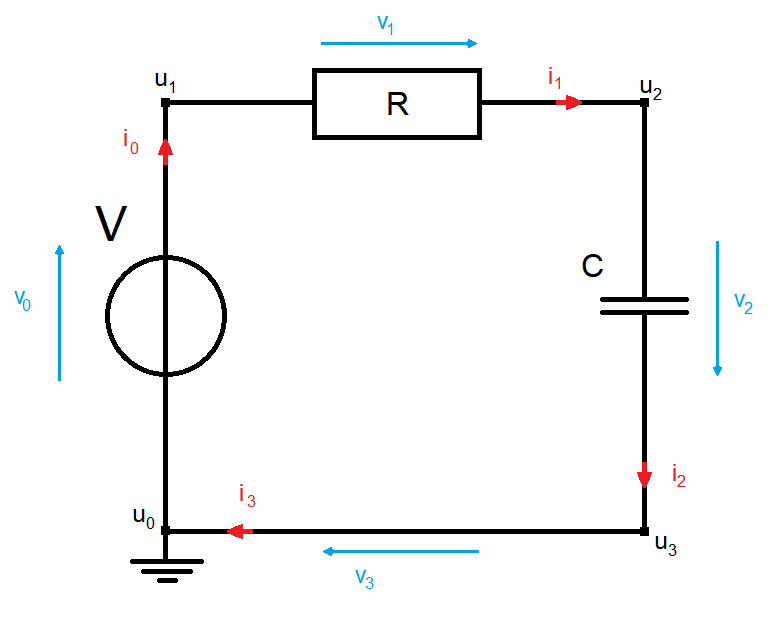
\includegraphics[scale=0.4]{../Tex/pictures/Example1_simple.png}
			\caption{charging capacitor with series resistor and voltage source}
			\label{circuit:charging of capacitor}
		\end{figure}
	\end{frame}

\section*{Formulating a Mathematical Model}

	\subsection{Network Topology}
		
	\begin{frame}
		\vfill
		For a circuit with $l$ nodes and $k$ edges, define the incidence matrix $\tilde{A} = (\tilde{a}_{ij}) \in \mathbb{R}^{k \times l}$:
		\begin{displaymath}
			\tilde{a}_{ij} = 
			\begin{cases}
				1 &   \text{edge $j$ starts at node $i$},\\
				-1 &  \text{edge $j$  ends at node $i$},\\
				0 & \text{else}.				
			\end{cases}
		\end{displaymath}
%		With 
%		\begin{align*}
%			\mathcal{N} = (n_0, n_1, n_2, ..., n_k) \quad &\cdots \quad \text{nodes},\\
%			\mathcal{E} = \{e_{j}: j = 1,...,l\} \quad &\cdots \quad \text{edges},
%		\end{align*}
%		furthermore
%		\begin{displaymath}
%			u = (u_0, u_1, u_2, ...) \quad \cdots \quad \text{corresponding electrical potentials at the nodes}.
%		\end{displaymath}
		By grounding node $0$, i.e. $u_0 = 0$ we obtain the reduced incidence matrix $\to$ $A$.
		\vfill
	\end{frame}

	\subsection{Energy Conservation Laws}
	\begin{frame}
		\vfill
		\begin{itemize}
			\item \textbf{Kirchhoff's voltage law (KVL):} \newline
			The sum of voltages along each loop of the network must equal to zero.
			\begin{equation}
				\label{KVL}
				\to A^\top  u = v.
			\end{equation}
			\item \textbf{Kirchhoff's current law (KCL):} \newline
			For any node, the sum of currents flowing into the node is equal to the sum of currents flowing out of the node.
			\begin{equation}
				\label{KCL}
				\to A  i = 0.
			\end{equation}
		\end{itemize}
		\vfill
	\end{frame}

	\subsection{Electrical Components and their Relations}
		
	\begin{frame}
		\vfill
		\begin{table}
			\centering
			\resizebox{\textwidth}{!}{
			\begin{tabular}{| c | c | c |}
				\hline
				\textbf{Name} & \textbf{Symbol} & \textbf{Component Law} \\
				\hline\hline
				Resistor & 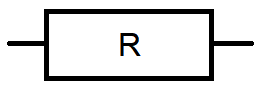
\includegraphics[height=0.9cm]{../Tex/pictures/resistor.png} & 	$v = R \ i \quad \text{or} \quad i = G \ u$ \\
				Capacitor & 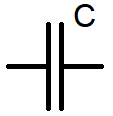
\includegraphics[height=1cm]{../Tex/pictures/capacitor.png} & $Q = C \ v \quad \text{and by derivation in t} \quad I = C \ \frac{d}{dt}v = C \ v'$ \\
				Inductor & 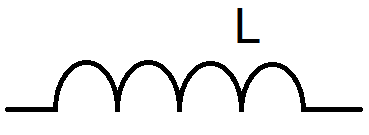
\includegraphics[height=0.9cm]{../Tex/pictures/inductance.png} & $\Phi = L \ i \quad \text{and by derivation in t} \quad v = L \ i'$ \\
				Voltage Source & 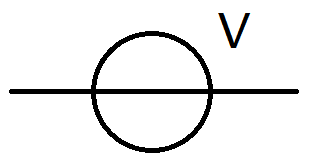
\includegraphics[height=1cm]{../Tex/pictures/voltage_source.png} & $v = v_{src}$ \\
				Current Source & 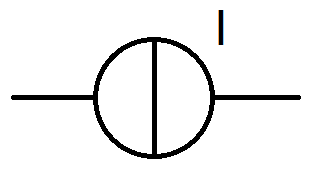
\includegraphics[height=1cm]{../Tex/pictures/current_source.png} & $i = i_{src}$ \\
				\hline
			\end{tabular}
			}	
		\end{table}
		\vfill
	\end{frame}
		
		
%	\begin{frame}
%		\begin{itemize}
%			\item \textbf{Resistor} \newline
%			\begin{equation}
%				\label{eq:resistor law}
%				v = R \ i \quad \text{or} \quad i = G \ u.
%			\end{equation}
%			\begin{figure}[H]
%				\label{fig:resistor symbol}
%				\centering
%				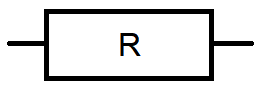
\includegraphics[width=2cm]{../Tex/pictures/resistor.png}
%				\caption{resistor symbol}
%			\end{figure}
%			
%			\item \textbf{Capacitor} \newline
%			\begin{equation}
%				\label{eq:capacitor law}
%				Q = C \ v \quad \text{and by derivation in t} \quad I = C \ \frac{d}{dt}v = C \ v'.
%			\end{equation}
%			\begin{figure}[H]
%				\label{fig:capacitor symbol}
%				\centering
%				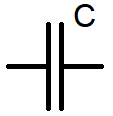
\includegraphics[width=2cm]{../Tex/pictures/capacitor.png}
%				\caption{capacitor symbol}
%			\end{figure}
%		\end{itemize}
%	\end{frame}
%			
%	\begin{frame}	
%		\begin{itemize}
%			\item \textbf{Inductor (Coil)} \newline
%			\begin{equation}
%				\label{eq:inductor law}
%				\Phi = L \ i \quad \text{and by derivation in t} \quad v = L \ i'.
%			\end{equation}
%			\begin{figure}[H]
%				\label{fig:inductor symbol}
%				\centering
%				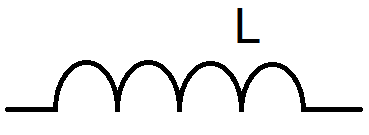
\includegraphics[width=3cm]{../Tex/pictures/inductance.png}
%				\caption{inductor symbol}
%			\end{figure}
%			
%			\item \textbf{Voltage Source} \newline
%			\begin{equation}
%				\label{eq:voltage source law}
%				v = v_{src}
%			\end{equation}
%			\begin{figure}[H]
%				\label{fig:voltage source symbol}
%				\centering
%				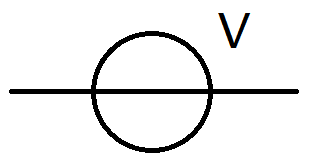
\includegraphics[width=4cm]{../Tex/pictures/voltage_source.png}
%				\caption{voltage source symbol}
%			\end{figure}
%		\end{itemize}
%	\end{frame}
%			
%	\begin{frame}
%		\begin{itemize}
%			\item \textbf{Current Source} \newline
%			\begin{equation}
%				\label{eq:current source law}
%				i = i_{src}
%			\end{equation}
%			\begin{figure}[H]
%				\label{fig:current source symbol}
%				\centering
%				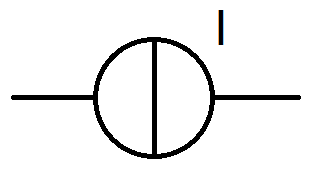
\includegraphics[width=4cm]{../Tex/pictures/current_source.png}
%				\caption{current source symbol}
%			\end{figure}
%		\end{itemize}
%	\end{frame}

	\subsection{Modified Nodal Analysis - MNA}
	\begin{frame}
		Rearrange the columns of the reduced incidence matrix $A$ into
		\begin{displaymath}
			A = (A_R A_C A_L A_V A_I)
		\end{displaymath}
		$A_R$, $A_C$, $A_L$, $A_V$ and $A_I$ ... columns related to components\\
		Represent voltages:
		\begin{displaymath}
			v = A^\top u
		\end{displaymath}
		$\to$ rearrange $v$ into $v = (v_R, v_C, v_L, v_{src}, v_I)$ and $i$ into $i = (i_R, i_C, i_L, i_V, i_src)$. 
		Rewrite component relations:
		\begin{align*}
			i_R = G \ v_R &= G \ A_R^\top u, \\
			i_C = C \ v'_C &= C \ A_C^\top u'.
		\end{align*}
		Kirchhoffs current law:
		\begin{displaymath}
			A_C i_C + A_R i_R + A_L i_L + A_V i_V = -A_I i_{src}.
		\end{displaymath}

	\end{frame}

	\begin{frame}
%		Together with component law for inductors \eqref{eq:inductor law} and potential-voltage relation for voltage sources \eqref{eq:voltage source law}:
		Combining the component relations with the reduced incidence matrix and the Kirchhoff's laws we get: 
		\begin{displaymath}
			\begin{aligned}
				A_C C A_C^\top u' + A_R G A_R^\top u + A_L i_L + A_V i_V &= - A_I i_{src} , \\
				L i_L'	- A_L^\top u &= 0 , \\
				-A_V^\top u &=  -v_{src}.
			\end{aligned}	
		\end{displaymath}
		In matrix form:
		\begin{equation}
			\label{MNA_Matrixform}
			\begin{pmatrix}
				A_C C A_C^\top & 0 & 0 \\
				0 & L & 0 \\
				0 & 0 & 0
			\end{pmatrix}
			*
			\begin{pmatrix}
				u' \\
				i_L' \\
				i_V'
			\end{pmatrix}
			+
			\begin{pmatrix}
				A_R G A_R^\top & A_L & A_V \\
				-A_L^\top & 0 & 0 \\
				-A_V^\top & 0 & 0 
			\end{pmatrix}
			*
			\begin{pmatrix}
				u \\
				i_L \\
				i_V
			\end{pmatrix}
			=
			\begin{pmatrix}
				-A_I i_{src} \\
				0 \\
				-v_{src}
			\end{pmatrix} . 
		\end{equation}
		$\to$ differential and algebraic variables
	\end{frame}

\section*{Differential Algebraic Equations}
	\subsection{Types of DAEs}
	\begin{frame}
		\vfill
		In the most general form a DAE can be written as:
		Find $y:\mathbb{R} \to \mathbb{R}^n$ such that
		\begin{equation}
			\label{Abstract_DAE}
			F(t, y(t), y'(t)) = 0, \qquad \forall t \in I
		\end{equation}
		
		with $F:\mathbb{R} \times \mathbb{R}^n \times \mathbb{R}^n \to \mathbb{R}^n$ sufficiently smooth and $I$ the time-interval.
		
		\textbf{Linear systems with constant coefficients} \newline
		find $y$ such that
		\begin{equation}
			\label{DAE-const-coeff}
			A y'(t) + B y(t) = f(t) ,
		\end{equation}
		with $A,B \in \mathbb{R}^{n \times n}$, $A$ singular, $B$ regular and $f:\mathbb{R} \to \mathbb{R}^n$ a function in time.
		$\to$ differential and algebraic variables
		\vfill
	\end{frame}
	
%	\begin{frame}
%		\begin{itemize}
%			\item \textbf{Linear systems with constant coefficients} \newline
%			find $y$ such that
%			\begin{equation}
%				\label{DAE-const-coeff}
%				A y'(t) + B y(t) = f(t) ,
%			\end{equation}
%			with $A,B \in \mathbb{R}^{n \times n}$, $A$ singular, $B$ regular and $f:\mathbb{R} \to \mathbb{R}^n$ a function in time.
%			
%			\item \textbf{Linear time dependent systems}
%			are systems of the form: find $y$ such that
%			\begin{displaymath}
%				A(t) y'(t) + B(t) y(t) = f(t) ,
%			\end{displaymath}
%			with $A, B:\mathbb{R} \to \mathbb{R}^{n \times n}$, $f:\mathbb{R} \to \mathbb{R}^n$ functions, $\forall t \in \mathbb{R}$: $A(t)$ is singular and $B(t)$ regular.
%			
%			\item  \textbf{Structured (non-linear) systems} \newline
%			are semi-explicit systems of the form: find $(y,z)$ such that
%			\begin{align}
%				y'(t) &= f(t, y(t), z(t)) , \\
%				0 &= g(t,y(t),z(t)) ,
%			\end{align}
%			with $f:\mathbb{R} \to \mathbb{R}^n$ and $g:\mathbb{R} \to \mathbb{R}^d$ functions.
%		\end{itemize}
%	\end{frame}

	\subsection{Weierstrass-Kronecker normalform}
	
	\begin{frame}
		\vfill
		\begin{definition}
			The matrix pencil $\{ A,B\}$ is called \emph{regular} if there exists some $c \in \mathbb{R}$, such that $(cA+B)$ is regular (i.e. $det(cA+B) \neq 0$), otherwise it is called singular.
		\end{definition}
		
			By applying equivalence transformations on the system matrices, we can transform the initial system into a system of the form
		\begin{equation}
			\label{transformed-DAE-const-coeff}
			\begin{aligned}
				u'(t) + Ru(t) &= s(t), \\
				Nv'(t) + v(t) &= q(t),
			\end{aligned}
		\end{equation}
		where $N$ is a nilpotent matrix and the matrix $R$ is regular.
		\vfill
%		\begin{theorem}[Jordan Normalform] %\protect{\cite[Theorem~13.2.1]{NumerikGewöhnlicherDifferentialgleichungen}}]
%			For every matrix $Q \in \mathbb{R}^{n \times n}$ there exists a regular matrix $T \in \mathbb{C}^{n \times n}$, such that
%			\begin{displaymath}
%				T^{-1}QT = J = diag(J_1, ..., J_r) \quad \text{with} \quad J_i = 
%				\left(
%				\begin{matrix}
%					\lambda_i & 1 & & 0 \\
%					0 & \lambda_i & \ddots & \vdots \\
%					& \ddots & \ddots & 1 \\
%					0 & \hdots & 0 & \lambda_i
%				\end{matrix}
%				\right)
%				\in \mathbb{C}^{m_i \times m_i}
%			\end{displaymath} 
%			and $n = m_1 + ... + m_r$.
%		\end{theorem}
	\end{frame}
	
%	\begin{frame}
%		\begin{theorem}[Weierstrass-Kronecker normalform]%[\protect{\cite[Satz~13.2.2]{NumerikGewöhnlicherDifferentialgleichungen}}]
%			\label{Kronecker-Normalform}
%			Let $\{ A,B \}$ be a regular matrix pencil. There exist $P,Q \in \mathbb{C}^{n \times n}$ such that
%			\begin{displaymath}
%				PAQ = 
%				\left(
%				\begin{matrix}
%					I_d & 0 \\
%					0 & N 
%				\end{matrix}
%				\right), \quad
%				PBQ = 
%				\left(
%				\begin{matrix}
%					R & 0 \\
%					0 & I_{n-d}
%				\end{matrix}
%				\right)
%			\end{displaymath}
%			where
%			\begin{displaymath}
%				N = diag(N_1, ..., N_r) \quad \text{with} \quad N_i = 
%				\left(
%				\begin{matrix}
%					0 & 1 & & 0\\
%					& \ddots &\ddots & \\
%					& & & 0 & 1 \\
%					0 & & & 0
%				\end{matrix}
%				\right)
%				\in \mathbb{R}^{n_i \times n_i}
%			\end{displaymath}
%			and R has Jordan Normalform. By $I_k$ we denote the identity matrix of size $k \times k$.
%		\end{theorem}
%		%Proof on blackboard
%	\end{frame}
	
%	\begin{frame}
%		using these findings:
%		Using the findings above we are able to transform the initial DAE \eqref{DAE-const-coeff} using the matrix $P$ from Theorem \ref{Kronecker-Normalform}. By multiplying with $P$ from the left, we obtain
%		\begin{displaymath}
%			P A y'(t) + P B y(t) = P f(t) .
%		\end{displaymath}
%		
%		Setting
%		\begin{displaymath}
%			y(t) = Q
%			\left(
%			\begin{matrix}
%				u(t) \\
%				v(t)
%			\end{matrix}  
%			\right) 
%			, \quad
%			Pf(t) = 
%			\left(
%			\begin{matrix}
%				s(t) \\
%				q(t)
%			\end{matrix}
%			\right),
%		\end{displaymath}
%		with $u(t),s(t) : \mathbb{R} \to \mathbb{R}^d$ and $q(t),v(t) : \mathbb{R} \to \mathbb{R}^{n-d}$.
%		
%		We get a system of the form
%		\begin{equation}
%			\label{transformed-DAE-const-coeff}
%			\begin{aligned}
%				u'(t) + Ru(t) &= s(t), \\
%				Nv'(t) + v(t) &= q(t),
%			\end{aligned}
%		\end{equation}
%		where $PAQ = 
%		\left( 
%		\begin{matrix}
%			I & \\
%			& N
%		\end{matrix} 
%		\right)$
%		and $PBQ = 
%		\left( 
%		\begin{matrix}
%			R & \\
%			& I
%		\end{matrix} 
%		\right)$.
%	\end{frame}
	
%	\begin{frame}
%		\begin{align}
%			\notag
%			v(t) &= q(t) - Nv'(t) = q(t) - N(\underbrace{q(t)-Nv'(t)}_{=v(t)})' = q-Nq'+N^2v'' \\ \notag
%			&= q-Nq'+N^2(q-Nv')'' = q-Nq'+N^2q''-N^3v''' \\ \notag
%			&\vdots \\ \notag
%			&= q-Nq'+...+(-1)^{k-1}N^{k-1}\underbrace{\frac{d^k}{dt^k}q}_{:=q^{(k-1)}}+(-1) \underbrace{N^kv^{(k)}}_{=0}\\ 
%			\label{solution-to-transformed-DAE-const-coeff-part2}
%			&= \sum_{i=0}^{k-1} (-1)^iN^iq^{(i)}(t)
%		\end{align}
%		where $k$ is the nilpotency index of $N$.
%	\end{frame}

	\begin{frame}
		\begin{definition}
			The nilpotency index $k$ of the matrix $N$ from the Weierstraß-Kronecker Normalform of a matrix pencil $\{A,B\}$ with $A$ singular is called the \emph{Kronecker-Index} of $\{A,B\}$, which we denote by $ind\{A,B\}$. Note that for $A$ regular we set $ind\{A,B\} = 0$.
		\end{definition}
		
		Auf Tafel oder auf slides: how to obtain that this means that for $k$ differentiations of the system we obtain an ODE.
	\end{frame}
	
	
	
	\subsection{Index of a Differential Algebraic Equation}
	
	\begin{frame}
		\begin{definition}%[differentiation index \protect{\cite[Definition~13.3.1]{NumerikGewöhnlicherDifferentialgleichungen}}]
			Consider the differential algebraic equation \eqref{Abstract_DAE} to be uniquely locally solvable and $F$ sufficiently smooth. For a given $m \in \mathbb{N}$ consider the equations
			\begin{displaymath}
				\begin{aligned}
					F(t,y,y') &= 0, \\
					\diff{F(t,y,y')}{t} &= 0, \\
					&\vdotswithin{=} \\
					\diff[m]{F(t,y,y')}{t} &= 0.
				\end{aligned}
			\end{displaymath}
			The smallest natural number $m$ for which the above system results in an explicit system of ordinary differential equations (ODEs), i.e. it has the form
			\begin{displaymath}
				y' = \phi(t,y),
			\end{displaymath}
			is called \textbf{differentiation index}.
		\end{definition}
	\end{frame}

	\begin{frame}
		\vfill
		\begin{definition}%[perturbation index \protect{\cite[Definition~13.3.3]{NumerikGewöhnlicherDifferentialgleichungen}}]
			Let $y(t)$ be the exact solution of \eqref{Abstract_DAE} and $\tilde{y}(t)$ be the solution of the perturbed system $F(t, \tilde{y}, \tilde{y}') = \delta(t)$. The smallest number $k \in \mathbb{N}$ such that 
			\begin{displaymath}
				\|y(t)-\tilde{y}(t)\| \leq C \left(\|y(t_0)-\tilde{y}(t_0)\|+\sum_{j=0}^{k}\max_{t_0 \leq \xi \leq T} \left\rVert 		\int_{t_0}^{\xi}\diff[j]{\delta}{\tau}(\tau)d \tau \right\rVert \right)
			\end{displaymath}
			for all $\tilde{y}(t)$, is called the \textbf{perturbation index} of this system.
		\end{definition}
		\vfill
	\end{frame}

\section*{Index Analysis of the Modified Nodal Analysis}
%	\subsection{General Index Analysis}
%	\begin{frame}
%		content...
%	\end{frame}
	\subsection{Topological Conditions}
	
	\begin{frame}
		\begin{itemize}
			\vfill
			\item The resulting equations have index $\nu \leq 2$, if the circuit neither contains loops of voltage sources nor cutsets of current sources.
			\item They have index $\nu \leq 1$, if the circuit contains neither loops of capacitors and/or voltage sources nor cutsets of inductors and/or current sources.
			\item They have index $\nu = 0$, if every node in the circuit is connected to the reference node (ground) through a path containing only capacitors.
			\vfill
		\end{itemize}
	\end{frame}

	\begin{frame}
		\vfill
		\begin{figure}
			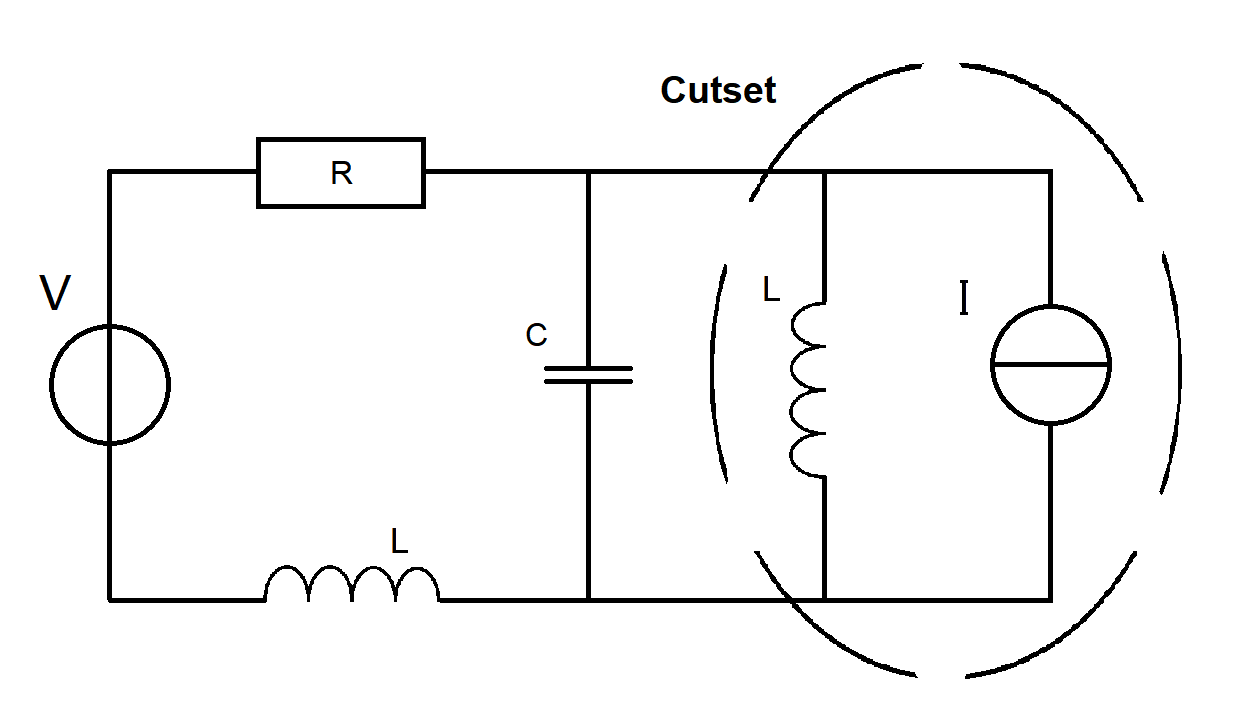
\includegraphics[width=0.475\linewidth]{../TeX/pictures/inductance-current-source_cutset.png}
			\hfill
			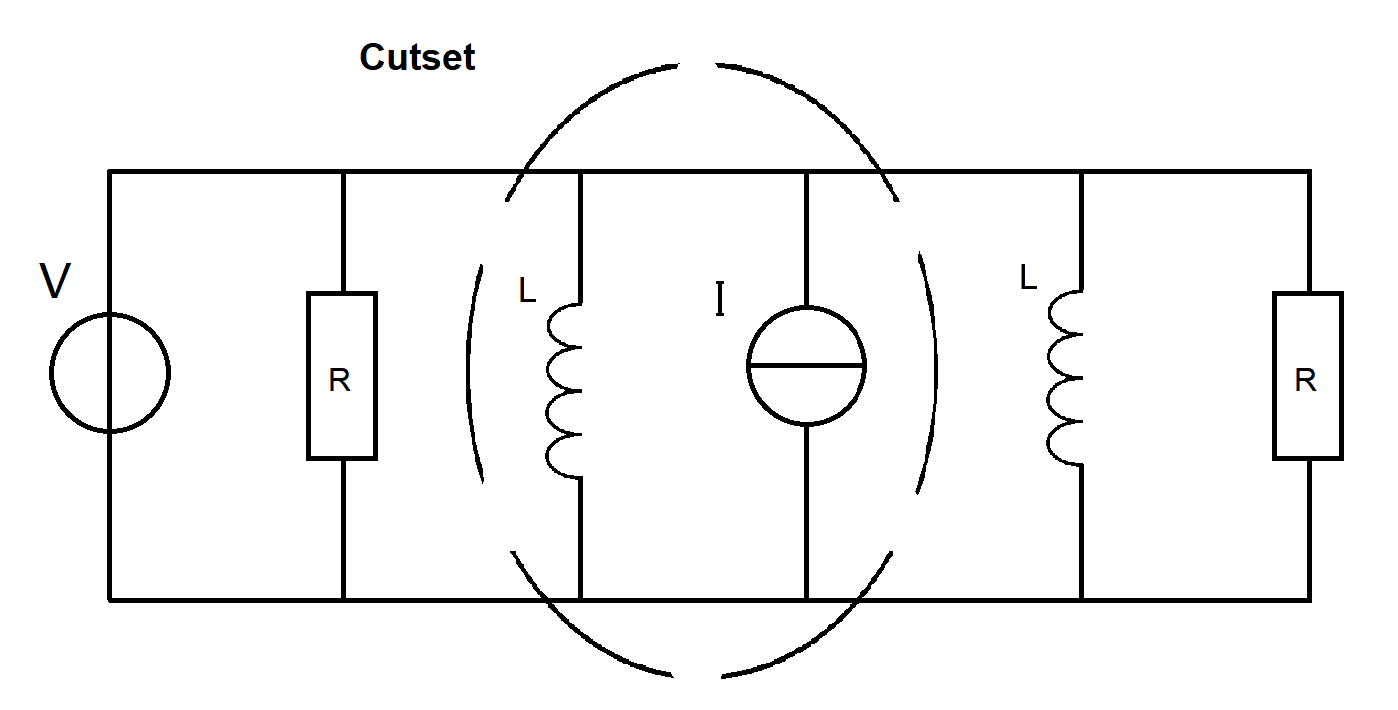
\includegraphics[width=0.475\linewidth]{../Tex/pictures/capacitance-voltage-source_loop.png}
			\caption{Illustration of a cutset and a loop.}
			\label{fig:cutset and loop}
		\end{figure}
		\vfill
	\end{frame}
	
	\begin{frame}
		\begin{theorem}[Index conditions] %\protect{\cite[Theorem~2.2.1]{shashkov_tuprints27452}}]
			Let the matrices of the capacitances, inductances and resistances be positive definite.
			\begin{itemize}
				\item If
				\begin{equation}
					\label{eq:index condition leq 2}
					ker([A_R, A_C, A_V, A_L]^\top) = \{0\} \quad \text{and} \quad ker(A_V) = \{0\}
				\end{equation}
				holds, then the MNA \eqref{MNA_Matrixform} leads to a system with index $\nu \leq 2$.
				
				\item If additionally
				\begin{equation}
					\label{eq:index condition leq 1}
					ker([A_R, A_C, A_V]^\top) = \{0\} \quad \text{and} \quad ker([A_C, A_V]) = \{0\}
				\end{equation}
				holds, then the system is of index $\nu \leq 1$
				
				\item If further
				\begin{equation}
					\label{eq:index condition eq 0}
					ker(A_C^\top) = \{0\} \quad \text{and} \quad dim(v_{src}) = 0
				\end{equation}
				holds, then the system has index $\nu = 0$.
			\end{itemize}
		\end{theorem}
	\end{frame}
	

\section*{Numerical Solutions}
%	\begin{frame}
%		general initial value problem
%		Find y, such that
%		\begin{align}
%			\label{general numerical problem}
%			y'(t) &= f(t,y), \quad t \in [t_0, t_l], \\
%			y(t_0) &= y_0.
%		\end{align}
%		
%		\begin{figure}[H]
%			\centering
%			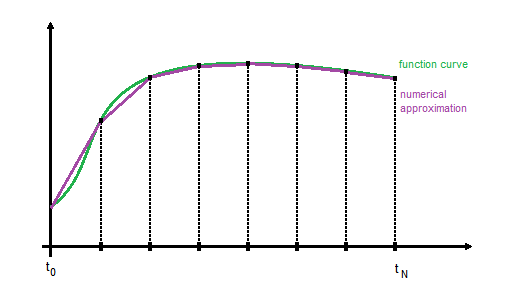
\includegraphics[scale=0.7]{../Tex/pictures/num_approx.png}
%			\caption{approximation of a function using numerical methods}
%			\label{fig:numerical approximation}
%		\end{figure}
%		
%	\end{frame}
%	\subsection{Single-Step Methods}
%	\begin{frame}
%		\begin{definition}
%			\label{def:single step mehod}
%			A numerical method to approximate a differential equation \ref{general numerical problem} on a time-grid $t_0,...,t_l$ with the intermediate values $y_0,...,y_l$ is called a single-step method if it is of the form
%			\begin{equation}
%				\label{single-step method}
%				y_{j+1} = y_j + h_j \phi(t_j,y_j, y_{j+1},h_j).
%			\end{equation}
%			We call $\phi$ the \emph{procedural function}. If $\phi$ does not depend on $y_{j+1}$, then the method is called \emph{explicit}, otherwise it is called \emph{implicit}.
%		\end{definition}
%	\end{frame}
	
%	\subsubsection{Consistency, Stability and Convergence}
%	\begin{frame}
%		\begin{definition}\label{Discretization_Error_SingleStep}
%			Let $y_{m+1}$ be the result of one step of a single step method \eqref{single-step method} with the exact start-vector $y_m = y(t_m)$ then
%			\begin{equation}
%				\label{local discretization error single step}
%				\delta_{m+1} = \delta(t_m+h) = y(t_{m+1}) - \tilde{y}_{m+1}, \quad m = 0,...,N-1
%			\end{equation}
%			is called the \emph{local discretization error} of the single step method at the point $t_{m+1}$.
%		\end{definition}
%	\end{frame}
%	
%	\begin{frame}
%		\begin{definition}\label{Consistency_SingleStep}
%			A single-step method is called \emph{consistent} if for all initial value problems \eqref{general numerical problem} 
%			\begin{equation}
%				\lim\limits_{h \to 0} \frac{\|\delta(t+h)\|}{h} = 0 \quad \text{for} \quad t_0 \leq t \leq t_l
%			\end{equation}
%			holds.\newline
%			It is called \emph{consistent of order p}, if for a sufficiently smooth function $f$
%			\begin{equation}
%				\|\delta(t+h)\| \leq Ch^{p+1} \quad \text{for all} \quad h \in \mathopen{(} 0,H \mathclose{]} \quad \text{and} \quad t_0 \leq t \leq t_l - h
%			\end{equation}
%			holds with $C$ independent of $h$.
%		\end{definition}
%	\end{frame}
%	
%	\begin{frame}
%		\begin{definition}\label{Convergence_SingleStep}
%			A single-step method is called \emph{convergent}, if for all initial value problems \eqref{general numerical problem} for the \emph{global discretization error}
%			\begin{displaymath}
%				e_m = y(t_m)-y_m
%			\end{displaymath}
%			holds that
%			\begin{displaymath}
%				\max\limits_{m}\|e_m\| \to 0 \quad \text{for} \quad h_{max} \to 0.
%			\end{displaymath}
%			The single-step method is called to have the \emph{convergence order} $p$, if
%			\begin{displaymath}
%				\max\limits_{m} \|e_m\| \leq C h_{max}^p \quad \text{for} \quad h_{max} \in \mathopen{(} 0,H \mathclose{]} \quad \text{with} \quad t_0 \leq t_m \leq t_l
%			\end{displaymath}
%			with the constant $C$ not dependent on the step size $h$.
%		\end{definition}
%	\end{frame}
%	
%	\begin{frame}
%		\begin{definition}\label{Discrete_Stability_SingleStep - lecture notes for numpdgl}
%			A single-step method is called \emph{(discretely) stable} if for grid-functions $y_h$ and $\tilde{y}_h$ with
%			\begin{align}
%				y_{i+1} &= y_i + h \phi(t_i, y_i), \\
%				\tilde{y}_{i+1} &=  \tilde{y}_i + h [\phi(t_i, \tilde{y}_i) + \theta_i],
%			\end{align}
%			and perturbations $\theta_i = \theta_h(t_i)$ of the right side as well as a bounded perturbation in the initial-values $y_0 - \tilde{y}_0$ the error is bounded by
%			\begin{displaymath}
%				\|y_h - \tilde{y}_h\|_{\infty,h} \leq C (\|y_0 - \tilde{y}_0\|_{l^2} + \|\theta_h\|_{\infty,h})
%			\end{displaymath}
%			with a constant $C$ which is not dependent on $h$. The norm $\|.\|_{\infty,h}$ denotes the maximum norm over the time-grid, i.e. for a function $b: T={t_0,...,t_N} \to \mathbb{R}^d$ we have $\|b\|_{\infty,h} = \max\limits_{t \in T}\|b(t)\|$, $\|b\|$ is the euclidean norm.
%		\end{definition}
%	\end{frame}
%	
%	\subsubsection{further stability properties}
%	
%	\begin{frame}
%		 Dahlquist equation, i.e. find $y$ such that
%		\begin{align}
%			y' &= \lambda y, \quad t > 0 \\
%			y(0) &= y_0
%		\end{align}
%		with $\lambda \in \mathbb{C}$ and $u_0$ fixed.
%	\end{frame}
%	
%	\begin{frame}
%		\begin{definition}
%			\begin{enumerate}
%				\item 
%				If a single-step method can be written in the form
%				\begin{equation}
%					y_{i+1} = R(z) \ y_i, \quad z:= h \lambda
%				\end{equation}
%				then we call $R: \mathbb{C} \to \mathbb{C}$ the \emph{stability function} of the single-step method.
%				\item 
%				The set
%				\begin{equation}
%					S := \{z \in \mathbb{C} : |R(z)| \leq 1\}
%				\end{equation}
%				is called the \emph{region of stability} of the method.
%				\item 
%				A single-step method is called
%				\begin{itemize}
%					\item \emph{0-stable}, if $0 \in S$.
%					\item \emph{A-stable}, if $\mathbb{C}^- \subset S$.
%					\item \emph{L-stable}, if $R(z) \to 0$ for $Re(z) \to -\infty$.
%				\end{itemize}
%			\end{enumerate}
%		\end{definition}
%	\end{frame}
	
	\subsection{Multistep Methods}
	\begin{frame}
		\vfill
		\begin{definition}[Multistep method]
			\label{def:multi step method}
			For given $\alpha_0, ..., \alpha_k$ and $\beta_0, ..., \beta_k$ the iteration rule
			\begin{equation}
				\label{linear-multistep-method}
				\sum_{l=0}^{k} \alpha_l y_{m+l} = h \sum_{l=0}^{k} \beta_l f(t_{m+l}, y_{m+l}), \quad m=0,1,...,N-k
			\end{equation}
			is called a \emph{linear multistep method} (linear k-step method). It is always assumed that $\alpha_k \neq 0$ and $|\alpha_0| + |\beta_k| > 0$. If $\beta_k=0$ holds, then the method is called explicit, otherwise implicit.
		\end{definition}
		\vfill
	\end{frame}
	
%	\subsubsection{Consistency, Convergence and Stability}
%	
%	\begin{frame}
%		\begin{definition}
%			Let $y_{m+k}$ be the result of one step of the multi-step method \eqref{linear-multistep-method} with the start-values given as the evaluations of the exact solution $y_{m+l} = y(t_{m+l})$ at $0 \leq l < k$. This means
%			\begin{displaymath}
%				\alpha_k \tilde{u}_{m+k} = \sum_{l=0}^{k-1} \left( h \beta_l f(t_{m+l}, y(t_{m+l})) - \alpha_l y(t_{m+l}) \right) + h \beta_k f(t_{m+k}, y_{m+k}) .
%			\end{displaymath}
%			Then
%			\begin{displaymath}
%				\delta_{m+k} = \delta(t_{m+k}) = y(t_{m+k}) - y_{m+k}, \quad m=0,1,...,N-k
%			\end{displaymath}
%			is called the \emph{local discretization error} (local error) of the linear multi-step method, see Def. \ref{linear-multistep-method} at the point $t_{m+k}$.
%		\end{definition}
%	\end{frame}
%	
%	\begin{frame}
%		\begin{definition}
%			A linear multi-step method is called %\emph{preconsistent} if for all functions $y(t) \in C^1[t_0,t_l]$
%			%		\begin{displaymath}
%				%			\lim\limits_{h \to 0} L[y(t),h]=0
%				%		\end{displaymath}
%			%		holds. 
%			%		It is called 
%			\emph{consistent}, if for all functions $y(t) \in C^2([t_0,t_l])$
%			\begin{displaymath}
%				\lim\limits_{h \to 0} \frac{1}{h} L[y(t),h] = 0
%			\end{displaymath}
%			holds. It has the \emph{consistency order p}, if for all functions $y(t) \in C^{p+1}[t_0, t_l]$
%			\begin{displaymath}
%				L[y(t),h] = \mathcal{O}(h^{p+1}) \quad \text{for} \quad h \to 0
%			\end{displaymath}
%			holds.
%		\end{definition}
%	\end{frame}
	
	\begin{frame}
		\vfill
		\begin{definition} \label{def: LMSM convergence}
			We say that a linear multi-step method is convergent, if for a solution $y$ of the problem and a vector $(y_j)_{j=0}^k$ created by an LMSM , we have that
			\begin{displaymath}
				\lim\limits_{h \to \infty} \max_{0 \leq j \leq k} ||y(t_j) - y_j|| = 0.
			\end{displaymath}
			If for $p \in \mathbb{N}$ and a constant $C$ not dependent on the step size $h$ we have
			\begin{displaymath}
				\max_{0 \leq j \leq k} ||y(t_j) - y_j|| \leq Ch^p,
			\end{displaymath}
			then we call the LMSM \emph{convergent with order $p$}.
		\end{definition}
		\vfill
	\end{frame}
	
%	\begin{frame}
%		\begin{definition} \label{discrete stability LMSM}
%			A linear multi-step method is called (discretely) stable, if for solutions $y_h$ and $\tilde{y}_h$ of
%			\begin{align}
%				\sum_{l=0}^{k} \alpha_l y_{m+l} &= h \sum_{l=0}^{k} \beta_l f(t_{m+l}, y_{m+l}), \\
%				\sum_{l=0}^{k} \alpha_l \tilde{y}_{m+l} &= h \sum_{l=0}^{k} \beta_l f(t_{m+l}, \tilde{y}_{m+l}) + h\theta_n
%			\end{align} 
%			and bounded initial values $y_j - \tilde{y}_j$ for $j \in {0,...,k}$ we have that
%			\begin{displaymath}
%				\max_{t_0 \leq t_n \leq T} ||y_n - \tilde{y}_n|| \leq C \sum_{j=0}^{k-1} ||y_j - \tilde{y}_j|| + \max_{t_0 \leq t_n \leq T} ||\theta_n||.
%			\end{displaymath}
%		\end{definition}
%	\end{frame}
	
	\subsubsection{further stability properties}
	
	\begin{frame}
		Dahlquist test problem as a model problem, find $y$ such that
		\begin{align}
			y' &= \lambda y, \quad t > 0 \\
			y(0) &= y_0
		\end{align}
		with $\lambda \in \mathbb{C}$ and $y_0$ fixed. \\
		Thus the resulting linear multistep method is of the form
		\begin{align*}
			\sum_{l=0}^{k} \alpha_l y_{n+l} = h \sum_{l=0}^{k} \beta_l \lambda y_{n+l} \\
			\iff \sum_{l=0}^{k}  [\alpha_l - h \beta_l \lambda] y_{n+l} = 0
		\end{align*}
	\end{frame}
	
	\begin{frame}
		\vfill
			\begin{definition}
			\begin{enumerate}
				\item 
				The set
				\begin{equation}
					\begin{aligned}
						S := \{z \in \mathbb{C} : \rho(\xi) - z \sigma(\xi) = 0 \implies \xi \in \mathbb{C} \text{ and } |\xi| \leq 1. \\
						\text{ If $\xi$ has multiplicity greater than $1$, then } |\xi| < 1\}
					\end{aligned}
				\end{equation}
				is called the region of stability of the method.
				\item 
				A linear multistep method is called
				\begin{itemize}
					\item \emph{0-stable}, if $0 \in S$.
					\item stable in the point $z \in \mathbb{C}$, if $z \in S$.
					\item \emph{$A(\alpha)$-stable}, if it is stable in all $z$ that lie within the set $\{z \in \mathbb{C}^- : |arg(z)-\pi| \leq \alpha\}$ for $\alpha \in (0, \frac{\pi}{2})$.		 
				\end{itemize}
			\end{enumerate}
		\end{definition}
		\vfill
	\end{frame}
	
	\begin{frame}
		\vfill
		\begin{theorem}%[\protecting{\cite[Satz~4.2.10]{NumerikGewöhnlicherDifferentialgleichungen}}]
			\label{th: null-stbaility and consistence is convergence}
			Let $f(t,y)$ be sufficiently smooth and the linear multi-step method be zero-stable and consistent of order $p$, then it is also convergent of order $p$.
		\end{theorem}
		\vfill
	\end{frame}
	
	\subsection{Consistent Initial Values}
	\begin{frame}
		\vfill
		\textbf{Index $\nu = 0$:} $\to$ arbitrary initial values since ODE.\\ 
		
		\textbf{Index $\nu = 1$:}\\
		
		By rewriting our system into the form
		
		\begin{align*}
			y'(t) = f(t,y(t),z(t)), \\
			0 = g(t,y(t),z(t)).
		\end{align*}
		
		we are able to give conditions for consistent initial values. Namely $y_0$ and $z_0$ are consistent initial values for this system, if $g(t_0, y_0, z_0) = 0$ holds.
		\vfill
	\end{frame}
	
	\begin{frame}
		\vfill
		\textbf{Index $\nu = 2$:}\\
		
		For index-2 systems we rewrite our system into
		
		\begin{align*}
			y' = f(t,y(t),z(t)), \\
			0 = g(t,y(t)).
		\end{align*}
		
		Consistent initial values $y_0$, $z_0$ for this case not only have to fulfill $g(t_0, y_0) = 0$ but also the \emph{hidden constraint} $g_t(t_0, y_0) + g_y(t_0, y_0)f(t_0, y_0, z_0)$. By $g_t$ and $g_y$ we denote the derivative of $g$ with respect to $t$ or $y$, respectively.
		\vfill
	\end{frame}
	
	\subsection*{Implicit Linear Multistep Formulas}
	
	\subsubsection{BDF-k Methods}
	
	\begin{frame}
		The \emph{backward differentiation formula (BDF)} is a family of implicit linear multistep methods. They have the general form
		\begin{equation}
			\sum_{k=0}^{s} \alpha_k y_{n+k} = h \beta f(t_{n+s}, y_{n+s})
		\end{equation}
		The BDF or BDF-k formulas for $k=1,...,3$ have the following form %or till 6
		\begin{align*}
			k = 1 &: h f_{m+1} = y_{m+1} - y_m \\
			k = 2 &: h f_{m+2} = \frac{1}{2} (3 y_{m+2} - 4 y_{m+1} + y_m) \\
			k = 3 &: h f_{m+3} = \frac{1}{6} (11 y_{m+3} - 18 y_{m+2} + 9 y_{m+1} - 2 y_m) %\\
			%		k = 4 &: h f_{m+4} = \frac{1}{12} (25 u_{m+4} - 48 u_{m+3} + 36 u_{m+2} - 16 u_{m+1} + 3 u_m) \\
			%		k = 5 &: h f_{m+5} = \frac{1}{260} (137 u_{m+5} - 300 u_{m+4} + 300 u_{m+3} - 200 u_{m+2} +75 u_{m+1} -12 u_m) \\
			%		k = 6 &: h f_{m+6} = \frac{1}{60} (147 u_{m+6} - 360 u_{m+5} + 450 u_{m+4} - 400 u_{m+3} + 225 u_{m+2} - 72 u_{m+1} + 10 u_m)
		\end{align*}
	\end{frame}
	
	\begin{frame}
		\begin{figure}[H]
			\centering
			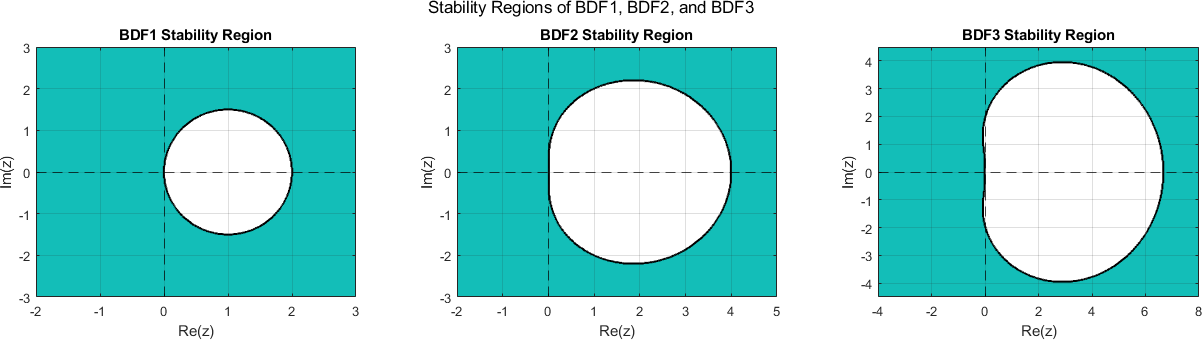
\includegraphics[width=0.8\linewidth]{../Tex/pictures/bdf_stability_regions.png}
			\caption{stability regions of BDF-schemes}
			\label{fig:screenshot020}
		\end{figure}
		\begin{theorem}%[\protecting{\cite[Satz~9.2.1]{NumerikGewöhnlicherDifferentialgleichungen}}]
			The BDF-k methods have consistency order $p=k$.
		\end{theorem}
		Using Theorem \ref{th: null-stbaility and consistence is convergence} we get that the BDF-k methods also have convergence order $p=k$.
	\end{frame}
	
	\subsubsection{Trapezoidal rule}
	
	\begin{frame}
		\vfill
		This procedure is repeated for small subsections of the interval $[a,b]$. Thus we obtain the iteration formula
		\begin{displaymath}
			u_h (t+h) = u_h(t) +\frac{h}{2}[f(t,u_h(t)) + f(t+h, u_h(t+h))].
		\end{displaymath}
		The trapezoidal rule, considered as a Lobatto~\RomanNumeralCaps{3}~A method, has convergence order $p=2$.
		\vfill
	\end{frame}
	
	
	
	\subsection*{Numerical Examples}
	
	\subsubsection{Example1}
	
	\begin{frame}
		\begin{figure}[H]
			\centering
			\begin{minipage}{.5\textwidth}
				\centering
				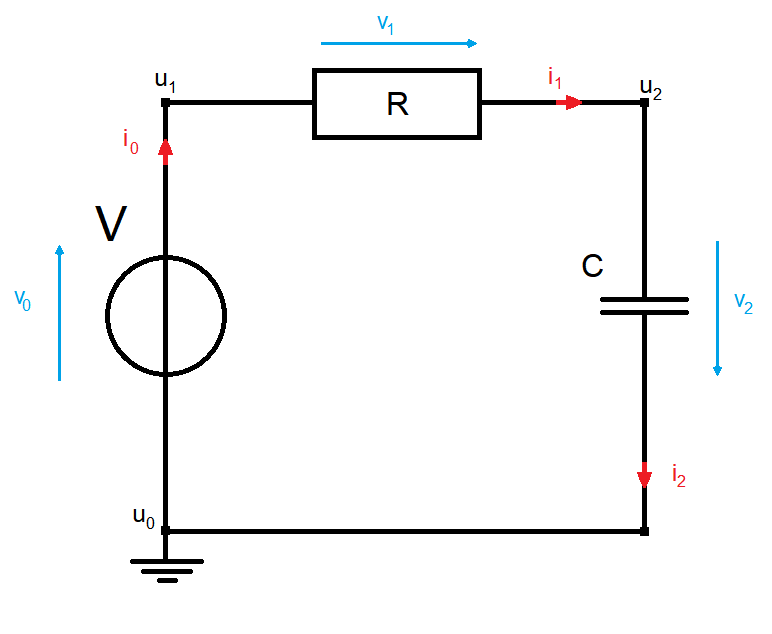
\includegraphics[width=\linewidth]{../Tex/pictures/Example1_simple_p2.png}
				\caption{charging capacitor with series resistor and voltage source}
				\label{fig:charging capacitor}
			\end{minipage}%
			\begin{minipage}{.5\textwidth}
				\centering
				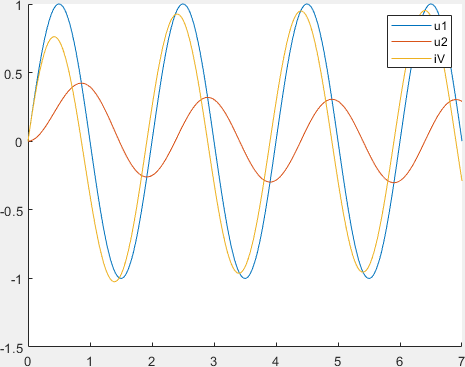
\includegraphics[width=\linewidth]{../Tex/pictures/exact_solution_ex1.png}
				\caption{Exact solution for example 1.}
				\label{fig: Exact solution for example 1}
			\end{minipage}
		\end{figure}
	\end{frame}
	
	\begin{frame}
		\vfill
		\begin{table}[H]
			\resizebox*{\textwidth}{!}{%
				\csvreader[tabular= | c || c c | c c | c c | c c |,
				table head = \hline h & \multicolumn{2}{c|}{k = 1} & \multicolumn{2}{c|}{k = 2} & \multicolumn{2}{c|}{k = 3} & \multicolumn{2}{c|}{trapezoidal}\\
				& u2 & iV & u2 & iV & u2 & iV & u2 & iV \\
				\hline,
				late after line=\\\hline]
				{../Matlab/err_ex1.csv}{h=\h, oneu=\oneu, oneuu=\oneuu, onei=\onei, twou=\twou, twouu=\twouu, twoi=\twoi, threeu=\threeu, threeuu=\threeuu, threei=\threei, trapu=\trapu, trapuu=\trapuu, trapil=\trapil}
				{\h  & \num{\oneuu} & \num{\onei}  & \num{\twouu} & \num{\twoi}  & \num{\threeuu} & \num{\threei}  & \num{\trapuu} & \num{\trapil}}
			}
			\caption{Resulting errors for the BDF-k methods and the trapezoidal rule.}
			\label{tab:num results ex1}
		\end{table}
		\vfill
	\end{frame}
	
%	\subsubsection{Example 2}
%	
%	\begin{frame}
%		\begin{figure}[H]
%			\centering
%			\begin{minipage}{.5\textwidth}
%				\centering
%				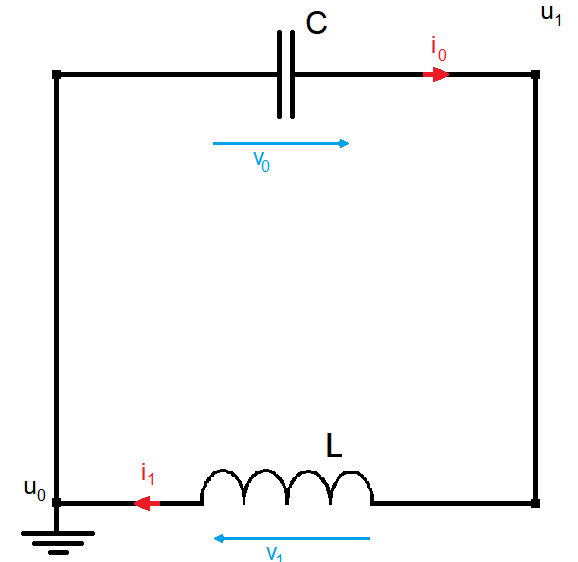
\includegraphics[width=\linewidth]{../Tex/pictures/Example2_index0.png}
%				\caption{LC-circuit}
%				\label{fig: LC-circuit}
%			\end{minipage}%
%			\begin{minipage}{.5\textwidth}
%				\centering
%				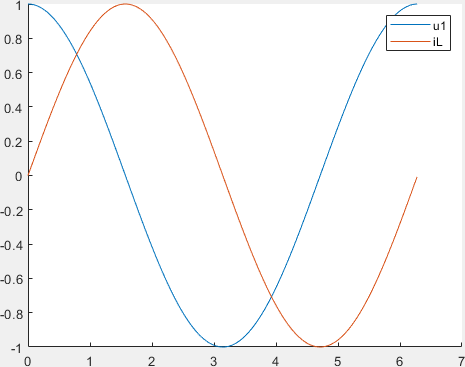
\includegraphics[width=\linewidth]{../Tex/pictures/exact_solution_ex2.png}
%				\caption{Exact solution for example 2.}
%				\label{fig: Exact solution for example 2}
%			\end{minipage}
%		\end{figure}
%	\end{frame}
%	
%	\begin{frame}
%		\begin{table}[H]
%			\resizebox*{\textwidth}{!}{%
%				\csvreader[tabular= | c || c c | c c | c c | c c | ,
%				table head = \hline h & \multicolumn{2}{c|}{k = 1} & \multicolumn{2}{c|}{k = 2} & \multicolumn{2}{c|}{k = 3} & \multicolumn{2}{c|}{trapezoidal} \\
%				& u1 & iL & u1 & iL & u1 & iL & u1 & iL \\
%				\hline,
%				late after line=\\\hline]
%				{../Matlab/err_ex2.csv}{h=\h, oneu=\oneu, onei=\onei, twou=\twou, twoi=\twoi, threeu=\threeu, threei=\threei, trapu=\trapu, trapil=\trapil}
%				{\h & \num{\oneu} & \num{\onei} & \num{\twou} & \num{\twoi} & \num{\threeu} & \num{\threei} & \num{\trapu} & \num{\trapil}}
%			}
%			\caption{Resulting errors for the BDF-k methods and ther trapezoidal rule.}
%			\label{tab:error ex2}
%		\end{table}
%	\end{frame}
%	
%	\subsubsection{Example 3}
%	
%	\begin{frame}
%		\begin{figure}[H]
%			\centering
%			\begin{minipage}{.5\textwidth}
%				\centering
%				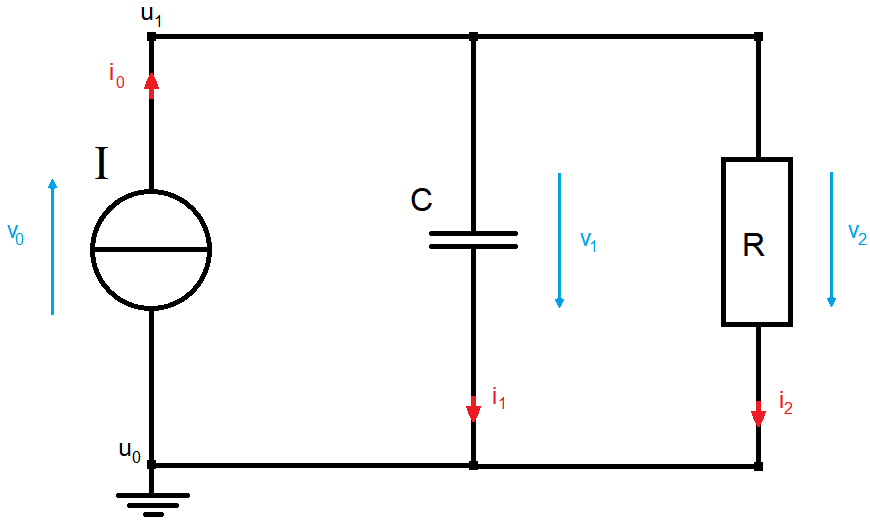
\includegraphics[width=\linewidth]{../Tex/pictures/Example3.png}
%				\caption{Current source with capacitor and resistor.}
%				\label{fig:num ex3}
%			\end{minipage}%
%			\begin{minipage}{.5\textwidth}
%				\centering
%				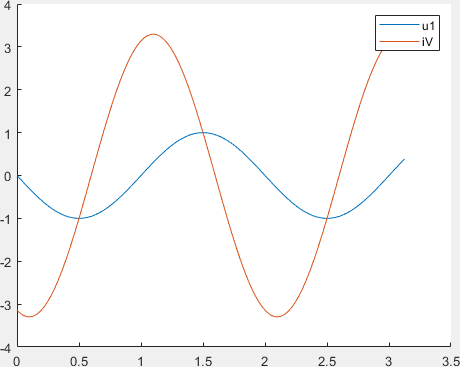
\includegraphics[width=\linewidth]{../Tex/pictures/exact_solution_ex3.png}
%				\caption{Exact solution for example 3.}
%				\label{fig: Exact solution for example 3}
%			\end{minipage}
%		\end{figure}
%	\end{frame}
%	
%	\begin{frame}
%		\begin{table}[H]
%			%\resizebox*{\textwidth}{!}{%
%				\centering
%				\csvreader[tabular= | c || c | c | c | c | ,
%				table head = \hline h & {k = 1} & {k = 2} & {k = 3} & trapezoidal \\ %\multicolumn{1}{c|}{}
%				& iV & iV & iV & iV \\
%				\hline,
%				late after line=\\\hline]
%				{../Matlab/err_ex3.csv}{h=\h, oneu=\oneu, onei=\onei, twou=\twou, twoi=\twoi, threeu=\threeu, threei=\threei, trapu=\trapu, trapil=\trapil}
%				{\h & \num{\onei} & \num{\twoi} & \num{\threei} & \num{\trapil}}
%				%}
%			\caption{Resulting errors for the BDF-k methods and the trapezoidal rule.}
%			\label{tab:error ex3}
%		\end{table}
%	\end{frame}